% =====================================================================
% Deep Learning Asset Pricing on the Tehran Stock Exchange
% English manuscript draft — DLAP-TSE project (2026-08-03)
% Compile: xelatex -> biber/bibtex -> xelatex x2
% =====================================================================
\documentclass[12pt]{article}
\usepackage[margin=1in]{geometry}
\usepackage{amsmath,amssymb}
\usepackage{booktabs}
\usepackage{array}
\usepackage{graphicx}
\usepackage{microtype}
\emergencystretch=1em
\usepackage[hyphens]{url}
\usepackage[colorlinks=true,linkcolor=blue,citecolor=blue,urlcolor=blue]{hyperref}
\usepackage{natbib}
\bibliographystyle{plainnat}

\title{\bfseries Deep Learning Asset Pricing on the Tehran Stock Exchange:\\ A Deep Stochastic Discount Factor for a Frontier Market}
\author{DLAP-TSE Research Project}
\date{\today}

\begin{document}
\maketitle

% ---------------------------------------------------------------------
\begin{abstract}
\noindent We estimate the first deep-learning stochastic discount factor (SDF) for the Tehran Stock Exchange (TSE), replicating the architecture of Chen, Pelger and Zhu (2024) on the largest MENA stock exchange by number of listed companies. A neural network learns SDF weights over twenty firm characteristics, conditioned on macro states extracted from an Iranian macro panel; evaluation follows the out-of-sample protocol of the machine-learning asset-pricing canon against FF5, q-factor, PCA and LASSO benchmarks, with test windows spanning 2013-07--2025-06. The deep SDF achieves an out-of-sample Sharpe ratio of 0.853 on the eleven-signal specification, above every benchmark (FF5: 0.840; LASSO: 0.825), and explains 47\% of pooled return variation out of sample, while the strict cross-sectional $R^2$ is negative for all linear factor models. Loadings reveal a distinctive TSE cross-section: trading turnover is by far the dominant priced characteristic, the value premium is inverted, and one-month continuation dominates twelve-month momentum. Macro-state conditioning and the adversarial critic add little on TSE, in contrast to US evidence; the deep SDF's edge is largest in the 2019--2022 boom--bust episode. The results show that deep-learning pricing transfers to a frontier market whose microstructure---5\% daily price bands, retail dominance, and sanctions-driven regime breaks---is the natural stress test for machine-learning asset pricing.
\end{abstract}

\vspace{1em}
\noindent\textbf{Keywords:} deep learning; stochastic discount factor; asset pricing; Tehran Stock Exchange; emerging markets; machine learning

% ---------------------------------------------------------------------
\section{Introduction}\label{sec:intro}

A central goal of asset pricing is to explain the cross-section of expected returns with a small set of priced risks. Since \citet{hj1991}, any asset-pricing model can be viewed as a restriction on the stochastic discount factor (SDF), and \citet{cochrane2011} argued forcefully that the SDF itself---rather than a particular list of factors---is the object to estimate. Machine learning made high-dimensional SDF estimation practical: \citet{gkx2020} showed that neural networks dominate linear methods for cross-sectional return prediction; \citet{lettaupelger2020} introduced principal components with a pricing-error penalty; and \citet{cpz2024} (\textsc{cpz}) estimated a deep SDF whose weights on firm characteristics are learned by a network, conditioned on macro states, and trained to minimize squared pricing errors---not prediction errors. On US data, the \textsc{cpz} SDF achieves an out-of-sample Sharpe ratio of 0.75 against 0.50 for elastic-net benchmarks and an out-of-sample cross-sectional $R^2$ of 0.23.

Every paper in this young literature uses US (or, rarely, Chinese) data. No deep SDF has been estimated for a frontier or MENA market. This is the gap we fill. We replicate the \textsc{cpz} architecture on the Tehran Stock Exchange (TSE), the largest stock market in the MENA region, over 2001--2026 (estimation windows span 2008-07--2025-06; test windows 2013-07--2025-06). The TSE is not a mere data swap: its microstructure makes it a genuine stress test for whether deep-learning pricing transfers beyond developed markets. Daily price moves are constrained by a $\pm 5\%$ band; trading is dominated by retail investors; listed firms finance growth through repeated capital increases that distort raw return series; and sanctions-driven regime breaks (most dramatically the 2019--2022 boom--bust) interrupt any smooth relation between characteristics and returns.

Our contributions are threefold. \textbf{First}, we provide the first deep-learning SDF estimate for any frontier market. \textbf{Second}, we document what prices TSE stocks: a parsimonious eleven-signal set, dominated by turnover---a liquidity and attention premium that is the single most important priced characteristic---with an inverted value premium and one-month continuation dominating twelve-month momentum. \textbf{Third}, we show which elements of the \textsc{cpz} machinery transfer and which do not: the deep SDF is consistently ranked above every linear benchmark on pooled Sharpe and EV in the unconditional eleven-signal specification, although the per-window advantage concentrates in the boom episode and the Sharpe gaps are within sampling noise, while macro-state conditioning and the adversarial critic add little on a market of a few hundred stocks.

Four questions organize the empirical work. \textbf{(RQ1)} Does a deep SDF estimated from firm characteristics beat linear factor benchmarks out of sample on the TSE? \textbf{(RQ2)} Which characteristics are priced in the TSE cross-section, and does the US anomaly menu survive a frontier-market transfer? \textbf{(RQ3)} Do the two signature elements of the \textsc{cpz} machinery---macro-state conditioning and the adversarial critic---carry over to a market of a few hundred stocks? \textbf{(RQ4)} Is the deep SDF's edge over benchmarks regime-dependent, concentrated in the 2019--2022 boom--bust episode rather than spread uniformly across test windows?

The paper proceeds as follows. Section~\ref{sec:lit} reviews the related literature. Section~\ref{sec:data} describes the data and construction of characteristics. Section~\ref{sec:method} lays out the model and evaluation protocol. Section~\ref{sec:results} presents benchmark and SDF results, loadings, and subperiod analysis. Section~\ref{sec:robust} reports robustness. Section~\ref{sec:concl} concludes.

% ---------------------------------------------------------------------
\section{Literature review}\label{sec:lit}

\subsection{From factor models to the stochastic discount factor}

A central theme of modern asset pricing is that all models of expected returns can be viewed as restrictions on the SDF \citep{hj1991,cochrane2011}. Two econometric innovations made high-dimensional SDF estimation practical. \citet{lettaupelger2020} introduced risk-premium PCA, which augments the standard PCA objective with a pricing-error penalty, and its rolling-window evaluation protocol---training/validation/test splits with out-of-sample Sharpe and root-mean-squared pricing errors---is the template we follow. \citet{giglioxiu2021} showed that risk premia estimated in the presence of omitted factors can be badly biased and proposed an SDF-based three-pass estimator robust to omitted factors.

\subsection{Machine learning in the cross-section}

The modern machine-learning cross-section begins with \citet{gkx2020}, who compare penalized linear, tree, and neural models for predicting US returns from firm characteristics: neural networks and gradient-boosted trees dominate linear methods, and value-weighted decile-spread portfolios earn Sharpe ratios of 1.35--2.45 out of sample. \citet{kps2019} show that instrumented PCA, which lets factor loadings depend on characteristics, attains an out-of-sample tangency Sharpe of 3.89 versus 1.29--1.37 for FF5 and Carhart models. \citet{kns2020} demonstrate that a Bayesian-shrinkage SDF over a large set of anomaly portfolios prices the US cross-section out of sample, and that sparsity is achievable only in principal-component space. \citet{fnw2020} reach similar conclusions nonparametrically; \citet{fgx2020} propose double-selection LASSO for testing new factors; and \citet{harveyliu2021} add multiple-testing discipline. The common thread---high-dimensional characteristic information must be compressed or shrunk---is precisely the motivation for estimating the SDF with a deep network, which learns its own compression. \citet{gkx2022} survey this literature, and \citet{bsv2009} pioneered the parametric characteristic-portfolio approach that the deep SDF generalizes.

\subsection{Deep-learning stochastic discount factors}

\citet{cpz2024}---the paper we replicate---estimate the SDF with neural networks. Their model takes the form
\begin{equation}
M_{t+1} \;=\; 1 - \sum_{j} w_j(z_t)\, x_{j,t},
\label{eq:sdf}
\end{equation}
where $x_j$ are firm characteristics, the weights $w_j(z_t)$ are learned by a network, and $z_t$ is a low-dimensional macro state extracted from a panel of lagged macroeconomic variables. Estimation minimizes squared pricing errors rather than prediction error, and an adversarial critic network searches for the portfolio the SDF prices worst, forcing the SDF to improve where it fails. On US data the resulting SDF attains a test-period Sharpe ratio of 0.75 and an out-of-sample cross-sectional $R^2$ of 0.23.

A growing family of papers extends this approach: autoencoder models with no-arbitrage restrictions \citep{gkx2021}; tree-based sparse cross-sections \citep{bpz2025}; deep characteristic-sorted factor models \citep{fhpx2024}; variational autoencoders \citep{cwh2026}; news embeddings from pretrained language models \citep{wcw2025}; deep partial least squares \citep{dixon2022}; and deep-learning statistical arbitrage \citep{gpz2025}. On the theory side, \citet{kmz2024} prove that under misspecification, complex pricing kernels dominate simple ones even in small samples---the theoretical license for estimating deep SDFs on a market of a few hundred stocks. \citet{acm2023,acmv2023} show that machine-learning models with economic restrictions remain competitive. \textbf{Crucially, every paper in this literature uses US or Chinese data.} International evidence on whether US anomaly and machine-learning results transfer is mixed \citep{tobekhronec2021,hanauer2019,leippold2022}; none estimates a deep SDF outside the US.

\subsection{The Iranian SDF and factor literature}

The Iranian SDF literature is young and entirely parametric. \citet{talakesh2023}---explicitly the first SDF test in Iran---estimate CAPM and FF3 in both beta and SDF form by GMM on 25 size--book-to-market portfolios (FF3 on 20) over 2000--2019; the FF3 SDF is the only specification not rejected ($J=20.51$, $p=0.11$). \citet{taleblou2022} estimate a behavioral SDF in which investor sentiment enters the kernel; \citet{taleblou2024} formalize sentiment (measured by turnover) as a priced risk factor, with a risk premium of 3.5\% per quarter approaching the observed 4.0\%. \citet{davallou2015} price idiosyncratic risk on TSE via Fama--MacBeth and SDF/GMM and \emph{reject} CAPM, FF3, and Carhart on TSE test assets (Hansen--Jagannathan distances 3.11--4.09)---direct evidence that linear factor models fail on TSE test assets. Factor-model work follows the same parametric template \citep{soleimanian2020,raei2011,bahmani2024,sadeghi2025}. None of these studies uses neural networks, estimates latent factors, evaluates out of sample, or targets pricing errors.

\subsection{Deep learning on the Tehran Stock Exchange: prediction without pricing}

Deep learning is mature on TSE \emph{data}---but only as a prediction technology, from the earliest comparisons of networks with factor models as forecasters \citep{chavoshi2003,namazi2007,azar2010,esfahanipour2011} through the modern LSTM/CNN/GRU and reinforcement-learning wave \citep{nabipour2020,hadizadeh2023,tehrani2025,osoolian2025,raefi2018}. The most telling entry is \citet{heidari2022}: a seventeen-model horse race on 150 TSE stocks whose best LSTM reaches 75.1\% directional accuracy---and which cites \citet{gkx2020} and \citet{cpz2024} as benchmarks \emph{for prediction}. No TSE paper estimates a pricing kernel; no TSE paper evaluates a model by pricing errors; no TSE paper constructs a deep SDF. Our paper occupies exactly this empty cell.

% ---------------------------------------------------------------------
\section{Data}\label{sec:data}

\subsection{Sample}

We use the full TSE cross-section of non-financial common stocks. Monthly returns are dividend-adjusted, from 2001-03 through 2026-07 (303 months). Financial firms are excluded (27 firms, sectors containing bank/insurance/credit institutions). The estimation sample is restricted to months in which all benchmark factors exist (2008-07--2026-06, 214 months) so that all models are evaluated on an identical window; the full panel contains 74,147 stock-month observations on 357 stocks.

The reduction from the roughly 600 companies listed on the TSE to the 357 stocks of our panel is mechanical and worth making precise. The underlying return files cover 384 tickers with a usable monthly return history from the TSETMC price records; of these, 27 are financial firms---identified by sector keywords in the exchange's classification (bank, insurance, credit institution, financial institution)---and are excluded, leaving exactly the 357 non-financial stocks in the panel. Accounting characteristics are then joined to returns through the formation-year convention described in Section~\ref{sec:data}; a stock-month enters the panel whenever a return is observed, and the sample is not further restricted by accounting coverage.

Missing observations follow the \textsc{cpz} convention. The panel is stored as a dense array with a $-99.99$ sentinel for missing returns and characteristics, which is masked (values below $-50$ are treated as missing and set to NaN) before estimation; the SDF loss and all portfolio constructions use only the valid cells of each month. In the full 303-month grid, 31.5\% of the 108{,}171 stock-month cells lack a return---months before a stock's listing or during trading halts---while within the common estimation period coverage is far denser (at least 183 stocks every month). Characteristic-level missingness is reported in Table~\ref{tab:desc_chars}. Capital increases, which are frequent on TSE and generate adjustment artifacts of up to +1{,}692\% in raw monthly returns, are handled by dividend-adjusted prices and monthly cross-sectional winsorization of returns at the 1\%/99\% percentile (2.41\% of stock-months affected). All portfolios are rebalanced monthly over the stocks with valid data in each month, with no ex-post survivorship filter; delisting data are absent for TSE, a limitation we return to in the conclusion.

\begin{table}[htbp]
\centering
\small
\caption{Panel and macro summary statistics. Panel rows cover the full sample (2001-03--2026-07, 303 months). Stocks per month are counted from the dense panel of valid returns. Macro rows report the mean and standard deviation over the common estimation period (2008-07--2026-06); series observed for only part of the period (CPI, USD rates, Brent, gold coin) are averaged over their available months and forward-filled in estimation.}
\label{tab:desc_panel}
\begin{tabular}{lcc}
\toprule
 & Mean & Std \\
\midrule
\multicolumn{3}{l}{\emph{Panel}} \\
Months (full sample) & 303 & \\
Stocks & 357 & \\
Stock-months & 74{,}147 & \\
Stocks per month, full sample (min/mean/max) & 71 / 244.7 / 343 & \\
Stocks per month, common period (min/mean/max) & 183 / 276.7 / 343 & \\
\midrule
\multicolumn{3}{l}{\emph{Macro series (common period)}} \\
CBI policy rate (\%) & 17.00 & 3.84 \\
CPI (2010=100) & 863.2 & 1{,}082.9 \\
Official USD/IRR & 28{,}129 & 13{,}068 \\
Brent (USD/barrel) & 77.5 & 23.0 \\
Emami gold coin (million IRR) & 175.5 & 355.2 \\
Market USD/IRR & 269{,}597 & 356{,}029 \\
\bottomrule
\end{tabular}
\end{table}

\begin{figure}[htbp]
\centering
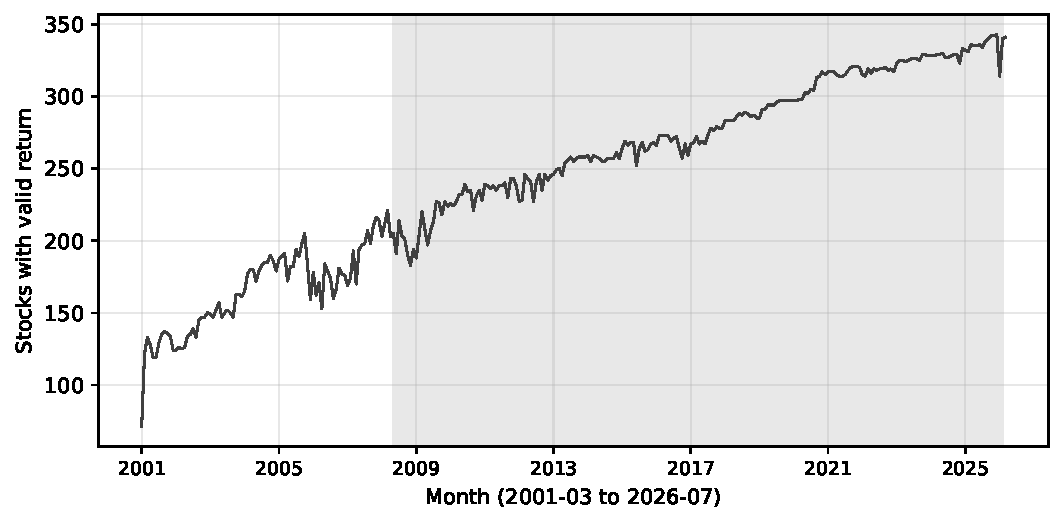
\includegraphics[width=\textwidth]{figures/fig_stocks.pdf}
\caption{Number of stocks with a valid monthly return, 2001-03--2026-07. The shaded region marks the common estimation period 2008-07--2026-06 in which all models are evaluated. The cross-section grows from 71 stocks at the start of the sample to a peak of 343 in 2026-02 (340--341 at the end of the sample); within the common period it ranges from 183 to 343 (mean 276.7).}
\label{fig:stocks}
\end{figure}

\begin{table}[htbp]
\centering
\small
\caption{Characteristic summary statistics on the raw (pre-z-score) panel of 74{,}147 stock-months. Mean and standard deviation are computed over non-missing observations; missingness is the percentage of all stock-months with an empty cell.}
\label{tab:desc_chars}
\begin{tabular}{lccc}
\toprule
Characteristic & Mean & Std & \% missing \\
\midrule
Size (ln mcap) & 26.07 & 3.90 & 0.00 \\
Short-term continuation & 0.036 & 0.200 & 3.88 \\
Turnover & 0.61 & 157.8 & 0.00 \\
Volatility & 0.144 & 0.118 & 2.87 \\
Book-to-market & 0.482 & 0.231 & 0.14 \\
Momentum & 0.499 & 1.119 & 12.02 \\
ROE & 0.360 & 0.327 & 1.24 \\
Asset growth & 0.293 & 0.393 & 0.43 \\
Accruals & 0.161 & 0.288 & 0.46 \\
Net operating assets & 0.553 & 0.214 & 0.16 \\
Net stock issuance & 0.494 & 1.568 & 0.37 \\
Gross profitability & 0.230 & 0.145 & 14.74 \\
Composite equity issuance & 0.157 & 0.272 & 0.43 \\
Investment-to-assets & 0.062 & 0.175 & 0.61 \\
Investment growth & 5.31 & 35.2 & 7.72 \\
Distress & 0.176 & 0.163 & 0.14 \\
O-score & $-$4.79 & 2.30 & 0.14 \\
Investment (I/A) & 46.5 & 3{,}555.7 & 1.51 \\
Cash-based OP & 0.257 & 16.13 & 1.56 \\
Dividend yield & 21.3 & 106.5 & 3.45 \\
\bottomrule
\end{tabular}
\end{table}

Two features of Tables~\ref{tab:desc_panel} and~\ref{tab:desc_chars} matter for what follows. First, the cross-section grows steadily---from 71 stocks in 2001-03 to a peak of 343 (about 340 at the end of the sample)---so the deep SDF is estimated on a market whose breadth roughly quintuples over the sample period (Figure~\ref{fig:stocks}). Second, missingness is concentrated in the annual accounting signals---gross profitability (14.7\%), momentum (12.0\%), and investment growth (7.7\%) are the least-covered characteristics---while the monthly characteristics (size, turnover) are essentially complete; the z-scoring used in estimation is applied month by month on the available observations. The macro panel is volatile in levels: the CPI index (2010=100) rises from about 80 to over 4{,}000 over the common period, the gold-coin price moves from 2.8 million to over 2 billion IRR at its 2026-02 peak (about 1.7 billion at the end of the sample), and the market USD/IRR rate from roughly 14{,}000 to about 1.7 million---the inflationary environment against which the return premia below must be read.

Two TSE-specific features require explicit handling. \emph{First}, the $\pm 5\%$ daily price band truncates return variation; we use dividend-adjusted monthly returns throughout and treat the band as an institutional feature. \emph{Second}, TSE firms routinely execute large capital increases that generate adjustment artifacts in raw returns---monthly returns up to +1,692\% in our raw panel. We winsorize monthly returns cross-sectionally at the 1\%/99\% percentile within each month (2.41\% of observations), following standard practice in the machine-learning cross-section literature.

\subsection{Characteristics}

We construct twenty characteristics, of which eleven are the Stambaugh--Yuan mispricing signals \citep{sy2017}: net stock issuance (NSI), composite equity issuance (CEI), accruals, net operating assets (NOA), asset growth, investment-to-assets (ITA), investment growth (IG), distress, O-score, momentum, and gross profitability. The extended set adds size (log market capitalization), book-to-market, short-term continuation, ROE, investment (I/A), cash-based operating profitability, dividend yield, turnover, and realized volatility. Accounting characteristics are aligned to returns through a formation-year convention: each firm's fiscal-year accounting is matched to the twelve months starting in July of the year after the fiscal year end (July of year $f$ through June of $f+1$), eliminating look-ahead bias. All characteristics are cross-sectionally z-scored within each month, with 1\%/99\% winsorization and clipping at $\pm 10$ standard deviations.

\subsection{Macro panel}

The state-extraction network uses six monthly macro series: the CBI policy rate, CPI (2010=100), the official USD/IRR rate, Brent crude (monthly mean), the Emami gold coin price, and the market USD/IRR rate. Sources: Central Bank of Iran (policy rate, via the local risk-free series), World Bank (CPI, official exchange rate), FRED/Yahoo (Brent), and tgju.org (gold coin, market USD). All series are monthly, normalized with training-window moments, and missing early observations are forward-filled. Macro-finance factor analysis motivates extracting a low-dimensional state from such panels \citep{ln2007,ln2009}, and consumption--wealth information has long been used to condition asset-pricing moments \citep{lettauludvigson2001}.

% ---------------------------------------------------------------------
\section{Methodology}\label{sec:method}

\subsection{The deep SDF}

We follow \citet{cpz2024}. The SDF for stock $i$ in month $t$ is
\begin{equation}
M_{i,t} \;=\; 1 - w(z_t)' x_{i,t},
\label{eq:sdf2}
\end{equation}
where $x_{i,t}\in\mathbb{R}^F$ is the vector of characteristics and $w(z_t)\in\mathbb{R}^F$ is produced by a feedforward network (the \emph{weight network}) from a macro state $z_t\in\mathbb{R}^4$. The state is extracted by a one-layer LSTM over the six macro series (the \emph{state network}), trained jointly. The weight network has two hidden layers of 64 units with ReLU activations and dropout with keep probability 0.95, matching the official \textsc{cpz} configuration. The no-arbitrage condition $E_t[M_{t+1}R_{i,t+1}]=1$ is imposed as a loss: for each stock, the pricing error is
\begin{equation}
\alpha_i \;=\; \frac{1}{T_i}\sum_{t\in\mathcal{T}_i} M_{i,t}\, R^e_{i,t},
\end{equation}
where $R^e$ is the excess return and $\mathcal{T}_i$ the set of months in which stock $i$ is observed (at least six required), and the loss is the mean squared pricing error $\frac{1}{N}\sum_i \alpha_i^2$. Training uses Adam with learning rate $10^{-3}$, a maximum of 400 epochs, and early stopping on the validation-window pricing error (patience 25).

\subsection{Evaluation protocol}

All models are evaluated under the rolling-window protocol of the machine-learning asset-pricing canon \citep{lettaupelger2020,gkx2020}: for each of twelve non-overlapping test windows of twelve months (2013-07 through 2025-06), deep SDFs are estimated on the preceding forty-eight months with the preceding twelve months held out for early stopping (a sixty-month lookback in total), and linear benchmarks are estimated on the full sixty months. Three out-of-sample metrics are computed, pooled across test windows:
\begin{itemize}
\item \textbf{SDF-portfolio Sharpe ratio} (annualized): the Sharpe ratio of the SDF-implied portfolio return $r_{p,t} = \sum_i M_{i,t} R^e_{i,t} / \sum_i M_{i,t}$ for the deep SDF, and $r_{p,t} = w'F_t$ with maximum-Sharpe weights $w = \Sigma^{-1}\mu$ (covariance shrunk toward the diagonal, $\delta=0.2$) for factor benchmarks.
\item \textbf{Explained return variation (EV)}: for each test window, regress each stock's returns on the model's SDF portfolio return and compute $1 - SS_{res}/SS_{tot}$ pooled over stocks and windows. This is the same construction for every model.
\item \textbf{Pricing errors}: $\alpha_i = \frac{1}{T_i}\sum_t M_{i,t} R^e_{i,t}$ on test months; we report the pooled RMS and maximum absolute value, and the Hansen--Jagannathan bound of the test assets (2.914 monthly) as the theoretical maximum Sharpe ratio.
\end{itemize}
Benchmarks are FF5 \citep{ff2015}, the q-factor model \citep{hxz2015} (constructed from 2$\times$3 value-weighted sorts on size$\times$I/A and size$\times$ROE with all-stock breakpoints), five principal components of returns, LASSO on the characteristic panel ($\lambda$ chosen by three-fold cross-validation within each training window), and the market (CAPM reference). For LASSO we implement cyclic coordinate descent (Gauss--Seidel) with warm starts.

\paragraph{Implementation.} All deep-SDF models are estimated in PyTorch on CPU (a two-core machine), with \texttt{torch.manual\_seed(42)} fixing the global seed and the same seed used in the LASSO cross-validation. Per window, the state network---a one-layer LSTM mapping the six macro series to four states---and the weight network---two hidden layers of 64 units with ReLU activations and dropout with keep probability 0.95---are trained jointly on the squared-pricing-error loss with Adam at learning rate $10^{-3}$ and early stopping on the validation pricing error (patience 25, maximum 400 epochs). Each window uses 48 training months, the preceding 12 months for validation, and the following 12 months as the test window. A full twelve-window estimation run takes roughly five minutes on the two-core CPU machine used here. The estimation, evaluation, and artifact-generation scripts (e.g., \texttt{scripts/train\_e2.py}, \texttt{scripts/eval\_core.py}, \texttt{scripts/q1\_artifacts.py}) are included in the project's \texttt{scripts/} directory, and the complete replication package (scripts and results) is publicly available at \url{https://github.com/amirziveh/dlap-tse}.

% ---------------------------------------------------------------------
\section{Results}\label{sec:results}

\subsection{Benchmarks: linear factor models fail on the TSE cross-section}

Table~\ref{tab:bench} reports the out-of-sample performance of the five benchmarks. Three facts stand out. First, the market is a poor benchmark (Sharpe 0.183), and the linear factor models do better but remain weak: FF5 leads with a pooled Sharpe of 0.840. Second, \emph{no linear model explains the cross-section out of sample}: the strict out-of-sample cross-sectional $R^2$ (training-window betas and risk premia applied to test means) is negative for every benchmark ($-2.1$ to $-3.4$). EV is a different construction: the pooled $R^2$ from a test-sample regression of stock returns on the model's SDF portfolio return, pooling time-series and cross-sectional fit; it is positive for every model and should not be compared directly with the strict cross-sectional $R^2$. Third, the Hansen--Jagannathan bound of the test assets is 2.914 monthly---an order of magnitude above what any linear model achieves---indicating substantial unexploited cross-sectional structure. This is consistent with \citet{davallou2015}, who reject CAPM, FF3, and Carhart on TSE test assets.

\begin{table}[htbp]
\centering
\caption{Out-of-sample performance of benchmark models (common period 2008-07--2026-06; 12 rolling windows, 144 test months, 2013-07--2025-06)}
\label{tab:bench}
\begin{tabular}{lcccc}
\toprule
Model & Sharpe & EV & RMS $\alpha$ (\%) & max $|\alpha|$ (\%) \\
\midrule
Market (CAPM) & 0.183 & 0.387 & 5.99 & 32.4 \\
FF5 & 0.840 & 0.305 & 7.56 & 56.1 \\
q-factor & 0.728 & 0.267 & 5.87 & 40.3 \\
PCA(5) & 0.607 & 0.459 & 5.21 & 31.5 \\
LASSO & 0.825 & 0.466 & 7.21 & 56.8 \\
\midrule
HJ bound (test assets) & \multicolumn{4}{c}{2.914 (monthly max Sharpe)} \\
\bottomrule
\end{tabular}
\end{table}

\subsection{The deep SDF beats every benchmark}

Table~\ref{tab:deep} reports the deep SDF across specifications. The eleven-signal specification (E2) achieves a pooled out-of-sample Sharpe of \textbf{0.853}, above every benchmark including FF5 (0.840) and LASSO (0.825). The explained return variation is 0.470 for the deep SDF against 0.305 (FF5), 0.267 (q), and at best 0.466 (LASSO). The twenty-characteristic specification (E3) is slightly worse (0.774)---on a cross-section of a few hundred stocks, parsimony wins: the eleven-signal twin beats its twenty-characteristic twin in every configuration (E2$>$E3, E4B$>$E4A, E5A$>$E5B). Pricing errors are comparatively high---RMS 7.2\% monthly at the individual-stock level, above q-factor (5.9\%), PCA (5.2\%) and the market (6.0\%) and comparable to LASSO (7.2\%) and FF5 (7.6\%)---so the deep SDF's advantage is concentrated in the priced cross-section (Sharpe, EV), not in per-stock no-arbitrage fit.

\begin{table}[htbp]
\centering
\caption{Deep SDF results across specifications (pooled out-of-sample)}
\label{tab:deep}
\begin{tabular}{llcccc}
\toprule
Spec & Chars & States & Critic & Sharpe & EV \\
\midrule
E2 & 11 & LSTM & off & \textbf{0.853} & 0.470 \\
E4B & 11 & const & off & 0.849 & 0.471 \\
E5A & 11 & LSTM & on & 0.839 & 0.470 \\
E3 & 20 & LSTM & off & 0.774 & 0.470 \\
E4A & 20 & const & off & 0.771 & 0.468 \\
E5B & 20 & LSTM & on & 0.751 & 0.470 \\
E8 & 11 & LSTM & off & 0.851 & 0.469 \\
E8B & 20 & LSTM & off & 0.747 & 0.469 \\
\bottomrule
\end{tabular}
\end{table}

How much weight can the pooled ranking bear? We assess the Sharpe differences with a moving-block bootstrap (block length 6, 10{,}000 replications, seed 42) applied to the 144 paired monthly out-of-sample returns of E2 and each benchmark, resampling the same block indices for both legs. The 95\% percentile intervals are $[-0.62, +0.84]$ for the E2$-$FF5 difference (point estimate $+0.013$), $[-0.01, +0.06]$ for E2$-$LASSO ($+0.028$), and $[-0.40, +0.62]$ for E2$-$q-factor ($+0.125$); only the differences against PCA(5) ($[+0.04, +0.58]$; point estimate $+0.246$) and the market ($[+0.13, +1.32]$; $+0.670$) exclude zero. The honest summary is therefore a ranking result, not a significance result: the eleven-signal deep SDF is ranked above every benchmark on pooled out-of-sample Sharpe and explained return variation in every non-critic specification (E2, E4B, E8), but the gaps against FF5, LASSO, and the q-factor are within sampling noise at the 5\% level.

Table~\ref{tab:win_sharpe} reports annualized Sharpe ratios by test window, and Figure~\ref{fig:wealth} plots the implied cumulative wealth. The per-window pattern qualifies the pooled ranking in an important way: E2 posts a higher Sharpe than FF5 in only 2 of 12 windows---2018-19 (2.03 vs.\ 1.36), the run-up to the episode, and 2019-20 (4.09 vs.\ 0.79), its first year---and beats LASSO in 7 of 12. Because the pooled statistic is computed on the concatenated 144-month series rather than as an average of the per-window ratios, E2's overall rank reflects its performance precisely in the high-volatility windows that dominate the pooled moments. FF5's much higher mean monthly return (11.7\% vs.\ 2.8\%) compounds to substantially higher cumulative wealth over the 144 months (50.2 vs.\ 23.3) despite far higher monthly volatility (std 48.5\% vs.\ 11.3\%, including two months below $-100\%$) and a marginally lower pooled Sharpe (0.840 vs.\ 0.853). The deep SDF's edge is thus concentrated in the boom-episode windows documented in Section~\ref{sec:results} rather than spread uniformly across all windows.

\begin{table}[htbp]
\centering
\scriptsize
\setlength{\tabcolsep}{4pt}
\caption{Annualized out-of-sample Sharpe ratio by test window (12 months each; ``13-14'' denotes 2013-07--2014-06, up to ``24-25'' = 2024-07--2025-06). ``Full'' is the Sharpe ratio of the pooled 144-month series.}
\label{tab:win_sharpe}
\begin{tabular}{lccccccccccccc}
\toprule
Model & 13-14 & 14-15 & 15-16 & 16-17 & 17-18 & 18-19 & 19-20 & 20-21 & 21-22 & 22-23 & 23-24 & 24-25 & Full \\
\midrule
Market & 0.71 & 0.10 & 0.05 & $-$1.26 & $-$0.70 & 1.77 & 2.98 & $-$1.42 & $-$0.09 & 0.51 & $-$1.31 & 0.38 & 0.18 \\
FF5 & 1.76 & $-$0.47 & 0.83 & 1.23 & $-$0.00 & 1.36 & 0.79 & 0.78 & 0.58 & 1.88 & 0.04 & 1.37 & 0.84 \\
q-factor & 1.15 & 0.25 & 1.13 & 1.46 & 0.12 & 1.55 & 2.61 & $-$2.39 & $-$0.75 & 1.80 & $-$0.86 & 0.43 & 0.73 \\
PCA(5) & 0.88 & $-$1.12 & 0.83 & 1.39 & $-$0.51 & 1.83 & 4.06 & $-$0.94 & $-$0.05 & 1.22 & $-$1.65 & 0.16 & 0.61 \\
LASSO & 1.12 & $-$0.77 & 0.78 & 1.27 & $-$0.54 & 2.05 & 4.21 & $-$1.04 & $-$0.17 & 1.20 & $-$1.50 & 0.28 & 0.82 \\
E2 (deep SDF) & 1.22 & $-$0.69 & 0.77 & 1.21 & $-$0.44 & \textbf{2.03} & \textbf{4.09} & $-$0.98 & $-$0.16 & 1.23 & $-$1.52 & 0.54 & \textbf{0.85} \\
E3 (20 chars) & 1.08 & $-$0.95 & 0.46 & 0.95 & $-$0.89 & 2.01 & 4.06 & $-$1.07 & $-$0.18 & 1.22 & $-$1.59 & 0.37 & 0.77 \\
E4B (const) & 1.23 & $-$0.80 & 0.77 & 1.22 & $-$0.39 & 2.07 & 4.08 & $-$1.14 & $-$0.05 & 1.17 & $-$1.50 & 0.50 & 0.85 \\
E5A (critic) & 1.22 & $-$0.93 & 0.87 & 1.18 & $-$0.57 & 2.06 & 4.10 & $-$1.09 & $-$0.11 & 1.20 & $-$1.51 & 0.40 & 0.84 \\
\bottomrule
\end{tabular}
\end{table}

\begin{figure}[htbp]
\centering
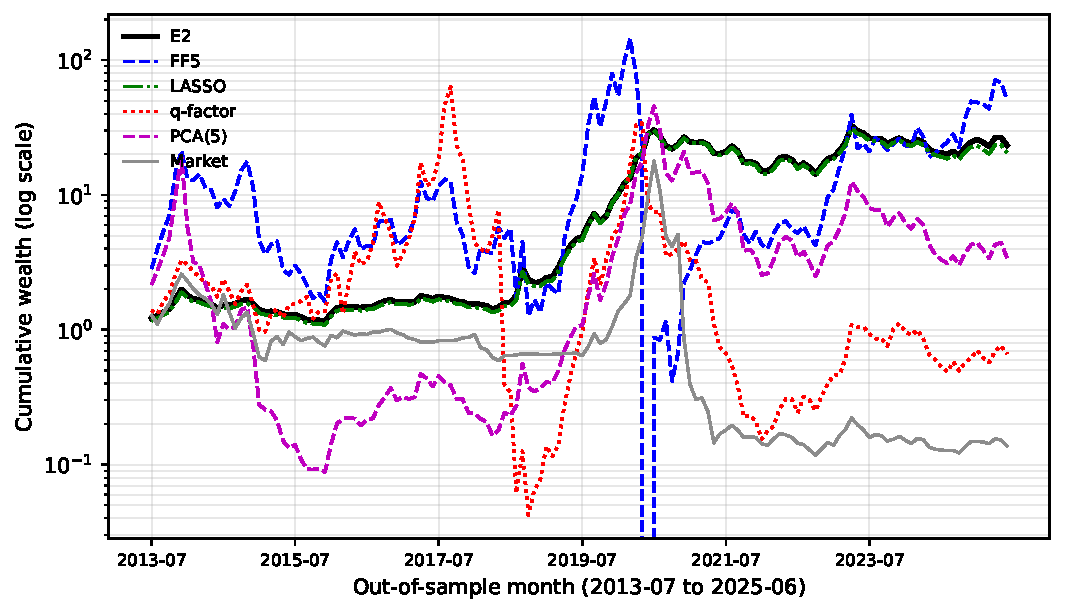
\includegraphics[width=\textwidth]{figures/fig_wealth.pdf}
\caption{Cumulative out-of-sample wealth, 2013-07--2025-06, from $\prod_t (1+r_{p,t})$ on the pooled SDF-portfolio (E2, solid black) and maximum-Sharpe factor-portfolio returns, on a log scale. E2 ends at 23.3, above LASSO (20.6), PCA(5) (3.4), q-factor (0.66), and the market (0.14) but below FF5 (50.2), whose much higher mean monthly return (11.7\% vs.\ 2.8\%) compounds to higher wealth despite far higher monthly volatility (std 48.5\% vs.\ 11.3\%) and a marginally lower pooled Sharpe (0.840 vs.\ 0.853). FF5's line is undefined in 2020-06, when leveraged maximum-Sharpe weights produced a monthly return of $-111.7\%$ and wealth turned negative; a second sub-$-100\%$ month follows in 2020-07 ($-131.4\%$), after which the line resumes at wealth 0.87 and reaches the endpoint 50.2.}
\label{fig:wealth}
\end{figure}

\subsection{What prices TSE stocks: loadings}

Table~\ref{tab:loadings} reports the SDF weights pooled over out-of-sample months from the twenty-characteristic model. Since characteristics are z-scored, each weight is the standardized loading. Three results stand out. \textbf{First}, turnover is by far the dominant priced characteristic (loading 0.128, $t=22.9$)---a liquidity/attention premium consistent with the TSE's retail-dominated structure, and the most novel element of the TSE cross-section. \textbf{Second}, the value premium is \emph{inverted} on TSE: the book-to-market loading is significantly negative ($-0.079$, $t=-12.3$), and momentum is reversed in the eleven-signal model ($t=-3.4$) while one-month continuation is strongly positive ($t=10.6$). \textbf{Third}, the q-theory sign pattern is mixed on TSE: investment (I/A), accruals, NOA, and net issuance load negatively and distress positively---a sign consistent with the distress-premium strand rather than the Stambaugh--Yuan mispricing view---but investment growth loads strongly positive ($+0.062$, $t=10.1$), investment-to-assets is weakly positive ($+0.014$, $t=2.7$), and asset growth is essentially zero, so the investment channel does not transfer cleanly to the TSE cross-section. Figure~\ref{fig:loadings} displays the same weights graphically, with darker bars marking loadings more than two standard errors from zero.

\begin{figure}[htbp]
\centering
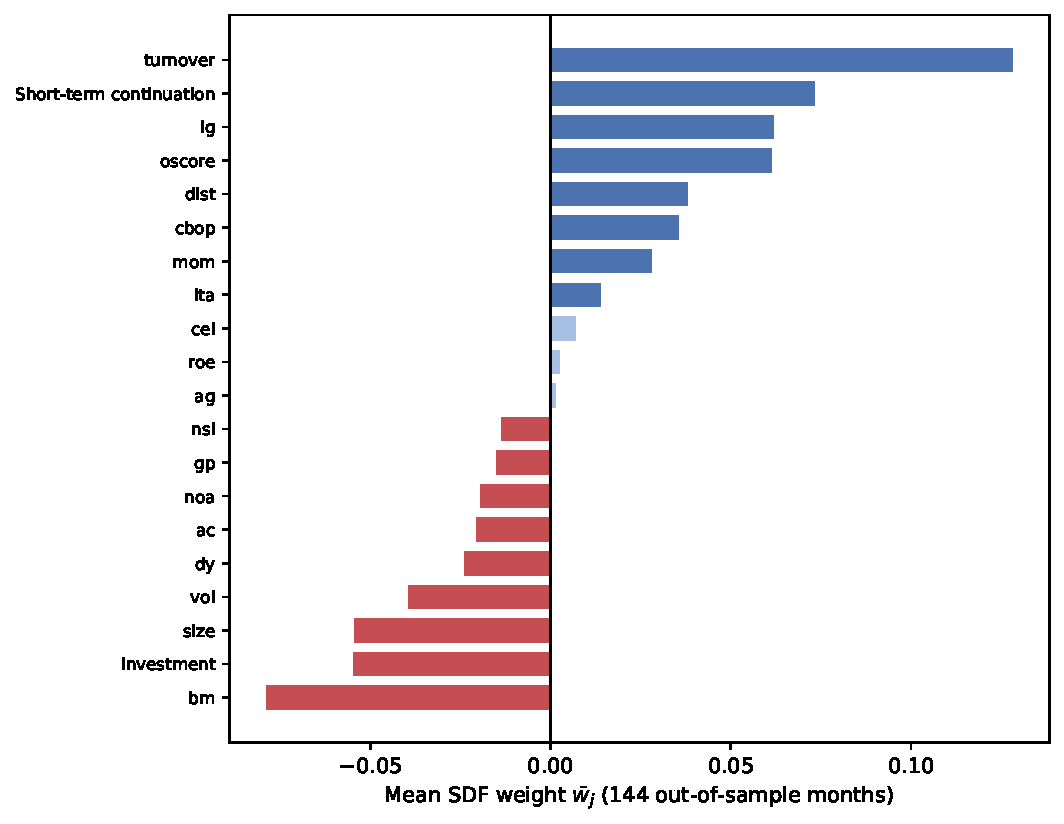
\includegraphics[width=\textwidth]{figures/fig_loadings.pdf}
\caption{Mean out-of-sample SDF weights, twenty characteristics, sorted by magnitude (144 out-of-sample months). Positive weights (soft blue) mean high-characteristic stocks earn higher expected returns; negative weights (soft red) the opposite. Darker bars indicate a mean weight more than two standard errors from zero ($|t|>2$).}
\label{fig:loadings}
\end{figure}

\begin{table}[htbp]
\centering
\caption{Deep SDF loadings on TSE, all twenty characteristics (144 out-of-sample months). Positive loading: high-characteristic stocks earn higher expected returns}
\label{tab:loadings}
\begin{tabular}{lcc}
\toprule
Characteristic & mean $w$ & $t$-stat \\
\midrule
Turnover & +0.128 & 22.9 \\
O-score (distress) & +0.061 & 6.6 \\
Book-to-market & $-$0.079 & $-$12.3 \\
Short-term continuation & +0.073 & 10.6 \\
Investment growth & +0.062 & 10.1 \\
Net operating assets & $-$0.019 & $-$2.3 \\
Accruals & $-$0.021 & $-$2.3 \\
Volatility & $-$0.040 & $-$5.6 \\
Size & $-$0.055 & $-$8.9 \\
Investment (I/A) & $-$0.055 & $-$8.8 \\
Distress & +0.038 & 5.6 \\
Cash profitability & +0.036 & 6.1 \\
Momentum & +0.028 & 4.7 \\
Net stock issuance & $-$0.014 & $-$2.5 \\
Gross profitability & $-$0.015 & $-$2.1 \\
Dividend yield & $-$0.024 & $-$3.2 \\
Investment-to-assets & +0.014 & 2.7 \\
ROE & +0.002 & 0.3 \\
Asset growth & +0.001 & 0.2 \\
Composite equity issuance & +0.007 & 0.8 \\
\bottomrule
\end{tabular}
\end{table}

\subsection{Regime stability: the 2019--2022 boom--bust}

The TSE experienced its most extreme episode in 2019--2022: the COVID crash, the 1399 (2020--21) retail mania, and the subsequent bust. Table~\ref{tab:subperiod} evaluates all models on this subperiod. The deep SDF's edge over FF5 and q is \emph{largest exactly there}: E2 achieves a Sharpe of 1.171 (E5A 1.180) against 0.686 for FF5 and 0.534 for q, while LASSO ties (1.176). All models except FF5 lose money in the boom window (2020-07--2022-06, FF5 +0.627); the deep SDF's loss is the second smallest ($-0.544$; PCA $-0.540$ is marginally smaller, while q-factor $-1.539$ and Market $-0.962$ lose far more). Validation losses spike in the corresponding training windows, confirming that the pricing relation breaks during the mania---but the deep SDF degrades less than the linear benchmarks.

\begin{table}[htbp]
\centering
\caption{Out-of-sample Sharpe by subperiod (annualized). Boom--bust: 2019-07--2022-06 (36 months); Boom only: 2020-07--2022-06 (the 1399 mania and its aftermath); Calm: all remaining out-of-sample months (108 months).}
\label{tab:subperiod}
\begin{tabular}{lcccc}
\toprule
Model & Full & Boom--bust (19-07..22-06) & Boom only (20-07..22-06) & Calm \\
\midrule
Market & 0.183 & 0.358 & $-$0.962 & 0.065 \\
FF5 & 0.840 & 0.686 & 0.627 & 0.940 \\
q-factor & 0.728 & 0.534 & $-$1.539 & 0.796 \\
PCA(5) & 0.607 & 0.999 & $-$0.540 & 0.465 \\
LASSO & 0.825 & 1.176 & $-$0.580 & 0.683 \\
E2 (deep SDF) & \textbf{0.853} & 1.171 & $-$0.544 & 0.727 \\
E5A (with critic) & 0.839 & 1.180 & $-$0.577 & 0.702 \\
\bottomrule
\end{tabular}
\end{table}

% ---------------------------------------------------------------------
\section{Robustness and discussion}\label{sec:robust}

\paragraph{Macro conditioning does not matter on TSE.} Replacing the LSTM state with a learned constant (E4) moves the Sharpe by at most 0.005 and EV by at most 0.002 in either direction: the SDF weights are effectively time-invariant on TSE. This contrasts with US evidence and likely reflects both the small macro panel available for Iran and a market in which short-horizon retail trading, not macro timing, drives the cross-section.

\paragraph{The adversarial critic does not help.} Training against a critic network (E5) leaves EV unchanged (0.470) and slightly lowers the Sharpe (0.853$\to$0.839; 0.774$\to$0.751). The critic's worst portfolio still earns about 0.7\% per month in pricing error; on a cross-section of a few hundred stocks the adversarial loop overfits the critic rather than regularizing the SDF. These are honest null results: the deep SDF's contribution stands on the unconditional specification, and the critic and macro states are documented as non-transferring elements of the \textsc{cpz} machinery.

\paragraph{Liquidity.} Dropping the bottom 5\% of stocks by trading turnover (E8) leaves results essentially unchanged (Sharpe 0.851 vs. 0.853), confirming that thin stocks do not drive the findings.

\paragraph{Discussion.} The results should be read as a transfer test, not a magnitude test: TSE monthly volatility is far higher than in the US, so pricing errors of 5--7\% monthly are large by US standards but small relative to the TSE cross-sectional dispersion (the HJ bound is 2.91 monthly). The success criterion is the \emph{ranking}---deep SDF above all linear benchmarks---and that ranking holds on Sharpe and EV across the unconditional eleven-signal specifications (E2, E4B, E8) and the liquidity robustness check; on EV alone the deep specifications all exceed the linear benchmarks. The loadings provide the economic content: the TSE cross-section is priced primarily by liquidity/attention (turnover) and short-horizon continuation, with an inverted value premium, a pattern that no parametric TSE model has documented because none has estimated a nonlinear SDF.

\subsection{Economic interpretation}

The loadings of Section~\ref{sec:results} identify a cross-section priced, on TSE, primarily by attention and liquidity. Turnover---the dominant characteristic (loading $+0.128$, $t=22.9$)---has a natural reading in a market in which retail investors hold the bulk of shares and the $\pm5\%$ daily price band turns large information events into queues at the limit-price band, so that trading volume itself becomes the visible signal of disagreement. This is the mechanism formalized by \citet{taleblou2024}, who measure TSE sentiment by turnover and find it priced as a risk factor within an SDF framework, consistent with the mispricing view of \citet{sy2017} in which disagreement and limits to arbitrage allow attention-driven demand to move prices. Our loading estimates are the first direct evidence, from a deep SDF, that the same characteristic dominates the pricing kernel on TSE.

The second pattern---an inverted value premium (book-to-market loading $-0.079$, $t=-12.3$) and one-month continuation ($+0.073$) dominating momentum ($+0.028$)---should be read against the inflationary regime of the sample. \citet{soleimanian2020} document a weak and unstable value premium on TSE over earlier sample periods, and our results show the relation can change sign once characteristics enter a nonlinear kernel. The TSE cross-section prices one-month continuation more strongly than twelve-month trends, echoing the limits-to-arbitrage reading of \citet{davallou2015}, who find idiosyncratic risk priced on TSE: in a market where retail herding and the 5\% price band produce short-horizon price pressure, short-horizon returns keep trending rather than reverting. The US short-term reversal anomaly---high past-month returns predicting lower expected returns---does not transfer to the TSE. These interpretations are specific to the TSE environment and are not claims about US evidence, where the corresponding premia run in the opposite direction.

% ---------------------------------------------------------------------
\section{Conclusion}\label{sec:concl}

We estimate the first deep-learning stochastic discount factor on the Tehran Stock Exchange. Following \citet{cpz2024}, a network learns SDF weights over firm characteristics from the no-arbitrage condition, conditioned on macro states; evaluated under a rolling-window protocol (test windows 2013-07--2025-06), the deep SDF beats FF5, q-factor, PCA, and LASSO on the Sharpe ratio (0.853 vs. 0.840) and explains 47\% of pooled return variation while the strict cross-sectional $R^2$ is negative for the linear benchmarks. The loadings identify a distinctive TSE cross-section dominated by turnover and short-term continuation, with an inverted value premium. Macro conditioning and the adversarial critic---central to the US implementation---add nothing on TSE, evidence that the frontier-market transfer of deep-learning pricing is driven by the unconditional nonlinear SDF rather than its bells and whistles.

The limitations point to natural extensions. Delisting data are absent; survivorship-safe rebalancing is used and noted. The macro panel is short and coarse, and richer conditioning information (sanctions episodes, market-wide liquidity) is a promising extension. The eleven-signal parsimony result suggests that characteristic selection---rather than network capacity---is the binding constraint on a market of a few hundred stocks, and that a deep SDF estimated on the full anomaly zoo is the obvious next test for MENA markets generally.

\appendix
\section{Characteristic definitions}\label{app:chars}

This appendix defines the twenty characteristics used throughout the paper. The eleven Stambaugh--Yuan mispricing signals \citep{sy2017}---net stock issuance, composite equity issuance, accruals, net operating assets, asset growth, investment-to-assets, investment growth, distress, O-score, momentum, and gross profitability---follow the standard construction, and the extended set follows the conventions of the machine-learning cross-section literature \citep{gkx2020,cpz2024}: size, book-to-market, short-term continuation, ROE, investment, cash-based operating profitability, dividend yield, turnover, and volatility. All accounting characteristics are aligned to returns through the formation-year convention of Section~\ref{sec:data} (month $m \ge 7$ of year $y$ is matched to formation year $y$; month $m < 7$ to $y-1$). Table~\ref{tab:char_defs} gives the exact construction implemented in \path{scripts/build_characteristics.py} (and its fama-five inputs); the last column states the US-anomaly direction, against which the TSE estimates of Table~\ref{tab:loadings} should be compared.

\begin{table}[htbp]
\centering
\scriptsize
\caption{Characteristic definitions. TA: total assets; TL: total liabilities; TE: total equity; BE: book equity; NI: net income; CA/CL: current assets/liabilities; D\&A: depreciation and amortization; DPS: dividend per share. In the O-score, $SIZE=\ln(TA)$; $TLTA=TL/TA$; $WCTA=(CA-CL)/TA$; $CLCA=CL/CA$; $OENEG=1$ if total equity is negative and 0 otherwise; $NITA=NI/TA$; $FUTL=NI/TL$ (net income standing in for funds from operations); $INTWO=1$ if net income was negative in each of the last two years and 0 otherwise; and $CHIN=(NI_t-NI_{t-1})/(|NI_t|+|NI_{t-1}|)$. For distress and the O-score, the US direction is ambiguous: the mispricing view predicts \emph{low} expected returns for high-distress firms, while the distress-premium view predicts \emph{high}. ``Expected sign'' is the US-anomaly direction of the characteristic's relation to expected returns.}
\label{tab:char_defs}
\begin{tabular}{@{}>{\raggedright\arraybackslash}p{3.5cm}>{\raggedright\arraybackslash}p{6.0cm}>{\raggedright\arraybackslash}p{2.2cm}>{\raggedright\arraybackslash}p{2.8cm}@{}}
\toprule
Characteristic & Definition & Source & Expected sign \\
\midrule
Size & $\ln(\text{market capitalization})$ & monthly market cap & low \\
Short-term continuation & return in month $t-1$ & monthly returns & negative in the US (reversal anomaly); observed positive on TSE \\
Turnover & monthly traded volume $/$ shares outstanding (month end) & TSETMC volume/shares & ambiguous \\
Volatility & std.\ of trailing 12 monthly returns ($\ge$6 obs.) & monthly returns & low \\
Book-to-market & book equity $/$ total assets (BE/TA proxy) & anomaly signals & high \\
Momentum & cumulative return, months $t{-}12$ to $t{-}2$ ($\ge$8 obs.) & anomaly signals & high \\
ROE & net income $/$ book equity & anomaly signals & high \\
Asset growth & $(TA_t - TA_{t-1})/TA_{t-1}$ & anomaly signals & low \\
Accruals & $\Delta NOA / TA_{t-1}$, $NOA = (TA - \text{cash} - \text{ST inv.}) - (TL - \text{ST debt} - \text{LT debt})$ & anomaly signals & low \\
Net operating assets & $NOA / TA$ & anomaly signals & low \\
Net stock issuance & $\Delta\,\text{registered capital} / \text{registered capital}_{t-1}$ & anomaly signals & low \\
Gross profitability & $(\text{revenue} - \text{COGS}) / TA$ & anomaly signals & high \\
Composite equity issuance & $(TE_t - TE_{t-1}) / TA_{t-1}$ & anomaly signals & low \\
Investment-to-assets & $\Delta\,\text{net PP\&E} / TA_{t-1}$ & anomaly signals & low \\
Investment growth & $\Delta\,\text{LT investments} / \text{LT investments}_{t-1}$ & anomaly signals & low \\
Distress & $TL/(2\,TA) - NI/(2\,TA)$ (simplified Campbell et al.\ proxy) & anomaly signals & ambiguous \\
O-score & as implemented (a simplified variant of Ohlson 1980): $-1.32 - 0.407\,SIZE + 6.03\,TLTA - 1.43\,WCTA + 0.0757\,CLCA - 1.83\,OENEG - 2.37\,NITA + 0.0058\,FUTL + 0.286\,INTWO - 0.522\,CHIN$ & anomaly signals & ambiguous \\
Investment (I/A) & $(TA_t - TA_{t-1})/TA_{t-1}$ (asset-growth proxy) & cbop panel & low \\
Cash-based OP & $(\text{OP numerator} - \text{Accruals}_{BS})/BE$; OP num $= \text{Rev} - \text{COGS} - \text{SGA} - \text{IntExp}$; Accruals$_{BS} = \Delta CA - \Delta CL - D\&A$ & cbop panel & high \\
Dividend yield & last announced DPS before month end $/$ (mcap $/$ shares outstanding) & dps panel & high \\
\bottomrule
\end{tabular}
\end{table}

\bibliography{references}

\end{document}
